\section[Who's data is it]{Let's talk about ownership}
\stepcounter{subsection} %We don't use subsection titles, only frametitles
\label{sec:ownership}

%---------------------------------------------------------------
% 1. Who's data is it?
%---------------------------------------------------------------
\begin{frame}{Who's data is it anyway?}

\begin{columns}[c]
    \begin{column}{0.45\textwidth}

    \begin{minipage}[t][.7\textheight]{\textwidth}

    Your creative output at work belongs to your employer.
    \begin{itemize}
    \item It is their \emph{Intellectual Property} (IP).
    \end{itemize}
    
    \vfill
    
    IP can take many forms:
    \begin{itemize}
        \item Formalised through patents, trademarks, copyright,...
        \item Also found in papers, presentations, photos, videos, audio,...
    \end{itemize}
    
    \vfill
    
    \textbf{Using IP without permission is ``IP Infringement'' (not good).}
    \end{minipage}%
    
    \end{column}

    \begin{column}{0.45\textwidth}
        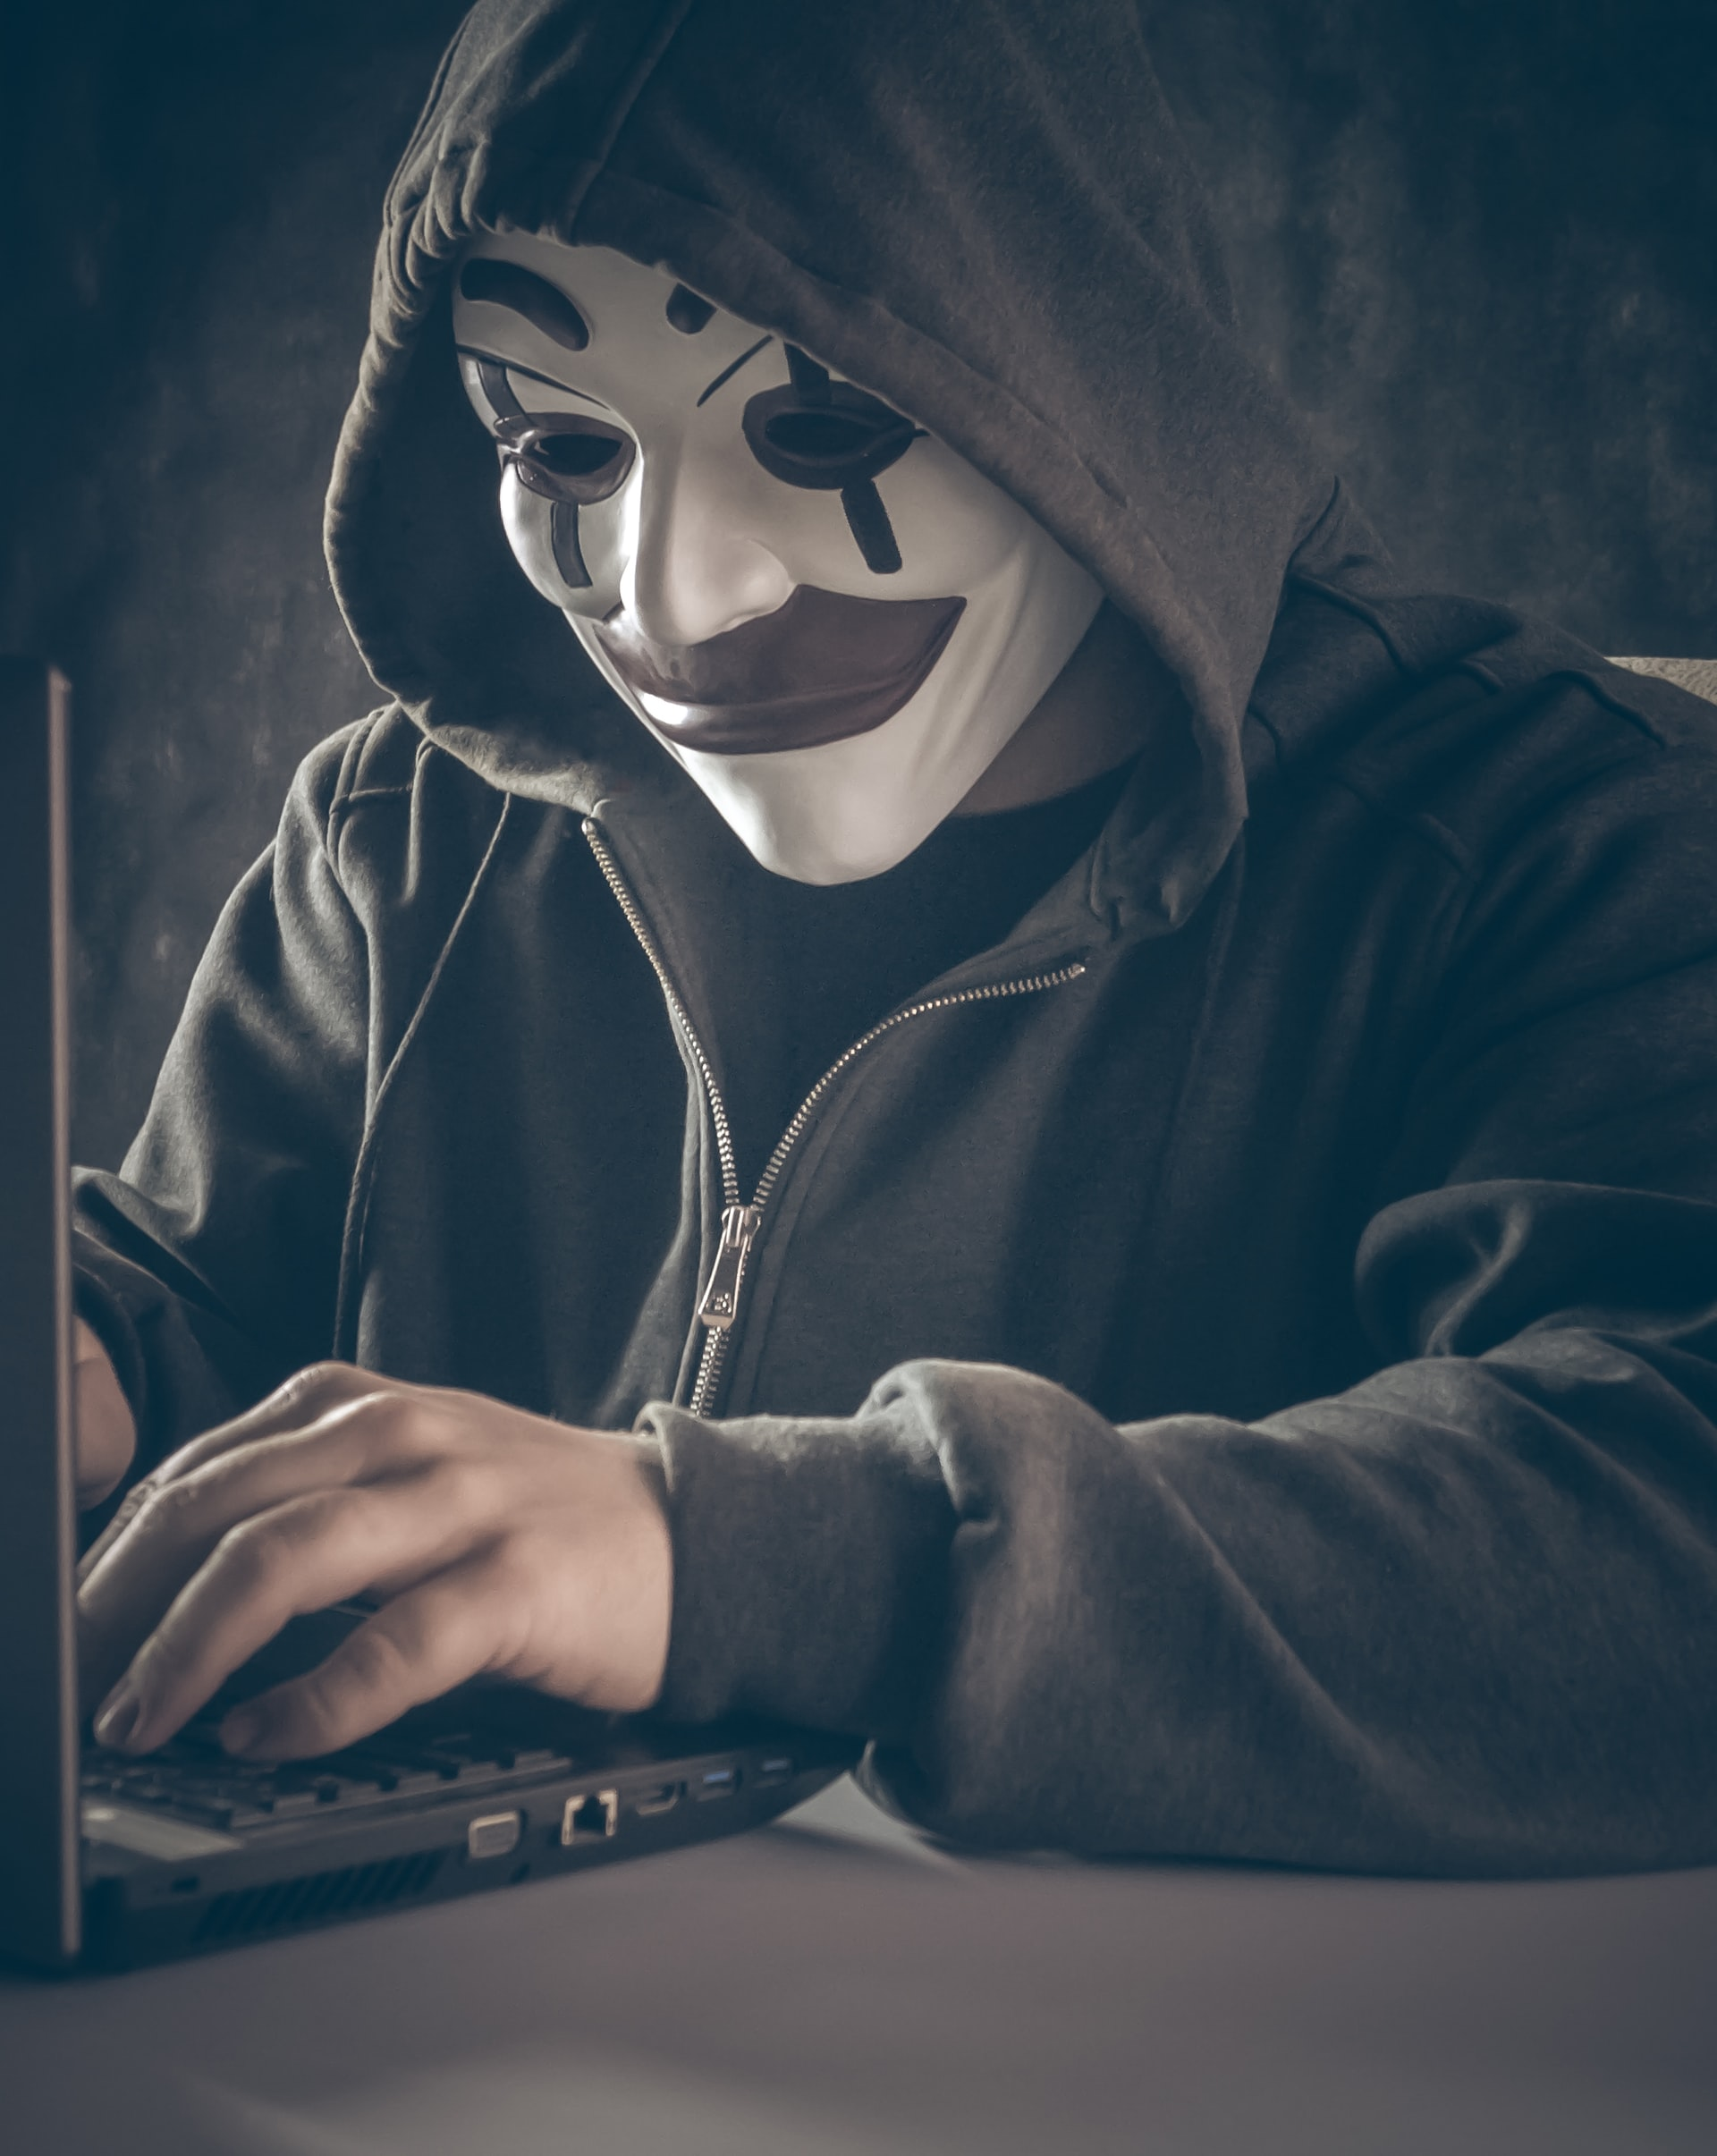
\includegraphics[width=0.85\textwidth]{images/bermix-studio-F7DAQIDSk98-unsplash.jpg}
        \givecredit{Photo by \textlink{https://unsplash.com/@bermixstudio}{Bermix Studio} on \textlink{https://unsplash.com/s/photos/thief}{Unsplash}}
    \end{column}

\end{columns}

\end{frame}

%---------------------------------------------------------------
% 2. How can I use it?
%---------------------------------------------------------------
\begin{frame}{This is where licenses come in}

\begin{columns}[c]

You need to talk to a lawyer

\end{columns}

\end{frame}

%---------------------------------------------------------------
% 3. What should we make open?
%---------------------------------------------------------------
\begin{frame}{What should we make open?}

\begin{columns}[c]
    \begin{column}{0.45\textwidth}

    Why do we 

    \end{column}
\end{columns}

\end{frame}
